\section{Four-interface transmission in an annulus}
\label{sec:annuli}

The continuum quantity used below is the probability that four interfaces
cross an annulus from one boundary component to the other.  Its existence
does not follow by applying the scalar Cardy hypothesis directly to a
multiply connected domain.  We establish it from the Jordan-domain inputs
of \cite{V}.  We also allow the boundary banks produced by stopped
explorations: a bank is viewed with its access from the domain, so distinct
banks may touch in the plane without being identified.

\subsection{Connection states and two caps}

Use the site triangulation drawn through the Voronoi tiling, with interface
strands drawn across the heterochromatic edges of its triangular faces.
These strands will be called \emph{walls}.  On a simple site cycle with
known colors, a \emph{run} is a maximal consecutive set of sites of one
color, and a \emph{switch} is the edge between consecutive runs.  Filling
the disk bounded by the cycle determines a noncrossing pairing of its switches by
walls.  The pairing, together with the run colors, determines connectivity
between boundary sites.  Closed walls need not be recorded.  We call this
pairing the connection state on the cycle.

Suppose each boundary component of a graph annulus has four switches and
four alternating prescribed runs.  All remaining sites have independent
fair colors.  Let $\mathcal T$ be the event that all four outer wall ends
reach the inner boundary.  There are two possible connection states in a
disk filling the inner cycle: the cap joining its two black runs, denoted
$\mathsf b$, and the cap joining its two white runs, denoted $\mathsf w$.
These are formal planar caps; no random colors are sampled in them.  Write
$H_{\mathsf b}$ and $H_{\mathsf w}$ for the indicators that the two outer
black runs are connected after the corresponding cap is attached.
Figure~\ref{fig:annular-caps} shows the two cap states when all four
walls are transmitted.

\begin{lemma}[The cap identity]\label{an:caps}
For every coloring of the annulus,
\begin{equation}\label{an:cap-equation}
 H_{\mathsf b}-H_{\mathsf w}=\mathbf 1_{\mathcal T}.
\end{equation}
Consequently the signed difference between the two inner cap states is
transferred to the same signed difference at the outer cycle, multiplied
by the indicator of four-interface transmission.  The identity remains
valid under composition across several cycles.
\end{lemma}

\begin{proof}
Walls in a triangulation neither branch nor cross.  If fewer than four
inner ends are connected to outer ends, the wall pairing visible from the
outer cycle is independent of the inner cap: there is no choice of pairing
on zero or two surviving ends.  Thus the left side of
\eqref{an:cap-equation} is zero.  If all four are transmitted, their cyclic
order is preserved, with any possible winding retained.  The intervening
monochromatic bands carry black connectivity to black connectivity and
white connectivity to white connectivity.  Hence $H_{\mathsf b}=1$ and
$H_{\mathsf w}=0$.  This is also the usual Hex duality proof after each run
is contracted to a vertex.  Composing the planar pairings proves the last
assertion; any closed walls created in the composition have weight one.
\end{proof}

\begin{figure}[tb]
\centering
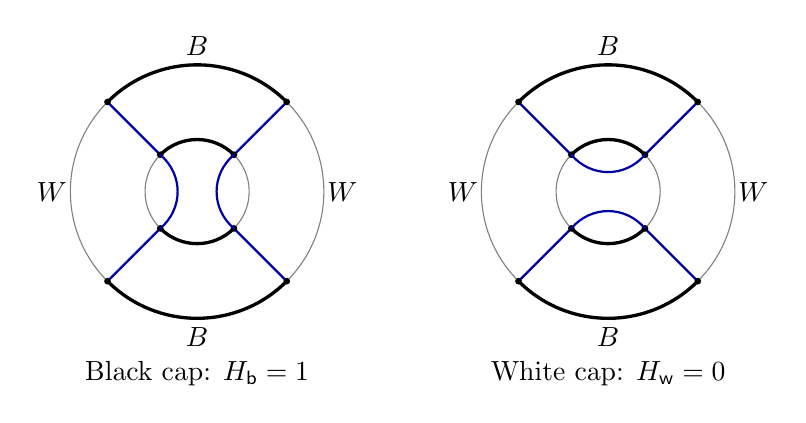
\begin{tikzpicture}[scale=0.87,line cap=round]
\foreach \a/\txt in {0/{Black cap: $H_{\mathsf b}=1$},6/{White cap: $H_{\mathsf w}=0$}} {
  \begin{scope}[xshift=\a cm]
    \draw[gray] (0,0) circle (1.85);
    \draw[gray] (0,0) circle (.76);
    \draw[very thick] (45:1.85) arc (45:135:1.85);
    \draw[very thick] (225:1.85) arc (225:315:1.85);
    \draw[very thick] (45:.76) arc (45:135:.76);
    \draw[very thick] (225:.76) arc (225:315:.76);
    \foreach \t in {45,135,225,315} {
      \draw[blue!65!black,thick] (\t:.76)--(\t:1.85);
      \fill (\t:.76) circle (1.4pt);
      \fill (\t:1.85) circle (1.4pt);
    }
    \node at (0,2.12) {$B$};
    \node at (0,-2.12) {$B$};
    \node at (-2.12,0) {$W$};
    \node at (2.12,0) {$W$};
    \node[align=center] at (0,-2.65) {\txt};
  \end{scope}
}
\draw[blue!65!black,thick] (45:.76) .. controls (.20,.25) and (.20,-.25) .. (315:.76);
\draw[blue!65!black,thick] (135:.76) .. controls (-.20,.25) and (-.20,-.25) .. (225:.76);
\begin{scope}[xshift=6cm]
\draw[blue!65!black,thick] (45:.76) .. controls (.25,.20) and (-.25,.20) .. (135:.76);
\draw[blue!65!black,thick] (225:.76) .. controls (-.25,-.20) and (.25,-.20) .. (315:.76);
\end{scope}
\end{tikzpicture}
\caption{The two cap pairings when all four walls are transmitted.
Blue curves are walls; thick black boundary arcs are black runs, and the
other runs are white.  The cap changes the outer black connection bit by
one.  The straight, unwound walls are schematic: the identity permits
winding and does not prescribe a pairing of numbered inner and outer
switches.}\label{fig:annular-caps}
\end{figure}

\subsection{The boundary convergence used below}

For $p>0$ let
\[
 \mathbb A_p=\{e^{-p}<|z|<1\}.
\]
Thus $p=\log(R/r)$ for a round annulus with radii $r<R$.  On both circles
angles increase counterclockwise.  Write $x=(x_1,x_2,x_3,x_4)$ for the outer
switches and $y=(y_1,y_2,y_3,y_4)$ for the inner switches, using increasing
lifts with $x_4<x_1+2\pi$ and $y_4<y_1+2\pi$.  Common translation of either
lift by $2\pi$ does not change the data.  The run following the first outer
switch is black.  For the $+$ prescription the corresponding inner run is
black; for the $-$ prescription it is white.

All limits in this section are taken along deterministic good sequences
of triangulations in the sense of \cite[Section 2, ``Deterministic
sequences and Jordan tests'']{V}.  In particular the mesh tends to zero on
compact sets, the joint Jordan-quad crossing limits hold, and the
mesh-first arm estimates recalled above are available.  Probabilities are
over product colors conditional on these triangulations.

\begin{definition}\label{an:admissible}
A sequence of marked graph annuli $D_n$ has \emph{admissible boundary
convergence} if it lies in a fixed bounded set and satisfies the following
conditions.
\begin{enumerate}
\item Each boundary is a simple site cycle.  With rotations normalized,
its uniformization
$\phi_n:\mathbb A_{p_n}\longrightarrow D_n$ extends continuously to the
closed annulus, where $p_n\to p\in(0,\infty)$.  After linear identification
in logarithmic radial coordinates, these maps converge uniformly on the
closed annulus to $\phi$.  The map $\phi$ is conformal and one-to-one in
$\mathbb A_p$, and its boundary traversal specifies the prime-end accesses
of $D=\phi(\mathbb A_p)$.
\item Each limiting boundary traversal is a concatenation of finitely
many simple arcs, each understood with its own access.  Different arcs
may meet in physical projection.  The two boundary components remain
distinct as prime-end boundary components.
\item The four switches on each component converge in these coordinates
to distinct switches.  Between them the prescribed run colors alternate.
The sites strictly between the two cycles have fresh independent fair colors.
\end{enumerate}
In graph constructions a boundary is taken without chords facing the
domain when that is required for a local boundary chart.  Such cuts are
obtained by the graph approximation and shortcut construction of
\cite[Section 2]{V}; at an exploration frontier, edges between already
revealed vertices are included before the frontier is taken.
\end{definition}

The definition permits a slit to have two different banks, even when
their images coincide.  It does not identify these banks.  The next
elementary convergence criterion explains how the domains arising from
stopped explorations fit this definition.

\begin{lemma}[A back with finitely many attached lobes]
\label{an:back-lobes}
Suppose graph annuli consist of an open annular back and finitely many
Jordan lobes attached to it along open seam intervals.  Assume that the
backs are Jordan annuli whose two complete boundary traversals converge
in curve order to those of a fixed Jordan annulus, the seam endpoints
converge in that order and the limiting seams remain open, and each lobe
converges as a Jordan domain with its boundary traversal.  The seam
incidences and cyclic order are fixed; lobes are glued only along their
specified seams, and their interiors are disjoint from the back and from
one another.  Suppose the resulting
limiting domain is an annulus, its hole and a separating open part of the
back persist, and the two boundary components stay physically apart.
Different limiting lobes may touch in projection but have disjoint
interiors.  Then the annular uniformizations converge uniformly on their
closures, with the stated accesses and traversal order.  In particular,
if the marked accesses converge and remain distinct, these domains have
admissible boundary convergence.
\end{lemma}

\begin{proof}
Every compact subset of a lobe persists by Jordan convergence.  The lobe
joins the back across every compact subinterval of its open seam.
Conversely, every point of the limiting boundary is approached by the
approximating boundaries.  Contacts between different lobes do not open
passages: the individual Jordan pieces are attached along their specified
seams, not through a point of contact.  These facts give kernel convergence
with the indicated accesses.  The persisting hole and separating back
exclude degeneration of the modulus.  The conformal kernel theorem
therefore gives convergence of normalized annular maps on interiors and
convergence of their moduli.

It remains to control the boundary parameters.  Fix a nonconstant open
subarc of one of the finitely many Jordan boundary pieces and a point in
the persisting back.  Jordan-map convergence in a lobe, or in a disk patch
along an unchanged back boundary, gives a positive lower bound for the
harmonic measure of a smaller subarc as seen from a point in that patch.
A Harnack chain through persisting interiors gives the same kind of lower
bound from the fixed back point.  In round annular coordinates the
harmonic-measure densities from its preimage are bounded above uniformly:
the moduli and the preimage stay in compact nondegenerate ranges.
Consequently no fixed nonconstant subarc of the boundary traversal can be
squeezed into an angular interval of length tending to zero.

The Jordan convergence of the finitely many pieces gives convergence of
the full boundary traversals in curve order.  Partition those traversals
into finitely many small image arcs, and apply the preceding lower bound
to intervening nonconstant subarcs.  A failure of equicontinuity in angular
parameters would traverse one such fixed subarc in a vanishing angular
interval, a contradiction.  This proves equicontinuity of the boundary
maps.  Interior convergence then identifies every uniformly convergent
subsequence, giving convergence on the closure.  Small crosscuts at the
finitely many joins give the same conclusion there.  There is no constant
boundary interval in the limiting conformal map, by uniqueness for a
holomorphic function continuous on a boundary arc.  The boundary order
and converging marked accesses thus also identify the limiting switches.
\end{proof}

\subsection{Boundary motion and annular crossing laws}

We first remove the rough banks.  The arm bounds needed here are
mesh-first statements: three free arms along one regular bank have an
upper bound with exponent $1+\eta$ for some $\eta>0$, and a free arm from a
shrinking neighborhood to a fixed scale has probability tending to zero.
The word \emph{free} excludes prescribed sites and cap wires.  The local
bank versions, including arms approaching the bank arbitrarily closely,
are those of \cite[Section 2, ``Cardy tests in a boundary chart'' and
``Free boundary-arm bounds'']{V}.

\begin{lemma}[Continuity under boundary motion]\label{an:motion}
For a sequence with admissible boundary convergence, move either cycle
slightly into the annulus in round coordinates, and move its switches
slightly with it.  Couple all unchanged free colors.  The probability
that either capped connection test changes tends to zero as the size of
the motion tends to zero, after taking the mesh limit.  The assertion also
holds for small piecewise smooth motions in spare space around an inset
annulus.  It is uniform along any convergent sequence of admissible data
with distinct limiting switches.  More precisely, if $H_n$ and
$H_{n,\delta}$ are either capped indicators before and after a motion of
size at most $\delta$, preserving the run order and its labels away from
the moving switches, then
\begin{equation}\label{an:motion-limit}
 \lim_{\delta\downarrow0}\limsup_{n\to\infty}
 \Pp(H_n\ne H_{n,\delta})=0.
\end{equation}
\end{lemma}

\begin{proof}
First the mesh in annular coordinates tends to zero.  Otherwise a
connected cell or triangle portion of vanishing physical diameter would
have preimages with a subsequential nontrivial continuum limit on which
$\phi$ is constant.  Such a continuum cannot meet the interior, where
$\phi$ is one-to-one, and cannot lie on the boundary, whose finitely many
simple arcs contain no constant interval.  Here graph portions, rather
than whole cells crossing the domain boundary, are used.

Remove small coordinate neighborhoods of the switches and of the
finitely many joins of simple bank arcs.  On each remaining compact bank
interval, use disk patches whose boundary consists of that bank and cuts
strictly inside the annulus.  Their physical boundaries are Jordan and
their graph approximations converge in curve order.  Their uniformizing
coordinates agree, with fixed-scale margins, with the annular coordinates;
reflection in the limiting round bank controls distortion on smaller
patches.  Thus the local boundary-arm estimates of \cite{V} apply on these
patches even when another prime-end bank has the same physical image.

Cover these intervals by $O(s^{-1})$ coordinate disks of radius $s$.
Implement a motion much smaller than $s$ by successively replacing bank
intervals, with tapered ends.  At graph level choose short transverse
joins in disjoint narrow strips from the old cycle to its replacement.
Substitute the intervals in cyclic order, retaining the old cycle off the
interval currently being changed and erasing the joins once the whole
cycle is replaced.  The graph approximation in curve order ensures that
these are simple cuts.  Each join has the same constant color as its run.
Moves containing switches or bank joins are instead included in the
exceptional neighborhoods.  Two nearby nonnested contours can be
compared through a common slightly inset contour.

Consider one ordinary move on a black bank.  If a capped connection test
changes, choose a winning black connection in one test and a winning
dual white connection in the other.  Contract the prescribed runs and
use the same cap in both tests.  Purely wired connections do not change,
so a free segment of a winning path must meet the support of the move.
The test neighborhood avoids every other run and mark.  The white path
has two free branches leaving that neighborhood.  At least one black
branch must also leave freely: a black branch already reaching the same
prescribed run outside the moved interval could be joined there without
the local change.  Taking simple paths after contraction gives disjoint
white branches, and the opposite-colored black branch is disjoint from
them in the common fair region.  This gives three free arms in a slightly
shifted half-patch, with fixed-factor margins.  The same argument applies
with the colors interchanged.  Forced sites on intermediate cuts are not
counted as free arms.

For any fixed larger chart scale, the mesh-first bound for a single disk
is $O(s^{1+\eta})$.  The union over $O(s^{-1})$ disks therefore costs
$O(s^\eta)$.  The number of exceptional neighborhoods is fixed.  A change
there requires a fair arm approaching from positive parameter distance:
connections already provided by the same run or by the cap do not
change.  This arm has positive physical diameter, uniformly after fixing
its outer parameter scale, by the no-continuum-fiber observation above.
The ordinary physical one-arm bound consequently makes the exceptional
cost tend to zero, including at a contact between different accesses.
One may move each exceptional neighborhood as a single piece, so this
cost is not multiplied by the number of ordinary intervals.

First take the mesh limit, then make the ordinary motions small compared
with $s$, then let $s$ tend to zero, and finally shrink the exceptional
neighborhoods.  This proves the assertion.  The same proof with moving
marks, or with a moving round radius, proves the stated continuity.
\end{proof}

After applying Lemma~\ref{an:motion}, all prescribed banks can be placed
on smooth contours strictly inside the parameter annulus, with spare
space on both sides.  There are still two separate issues: joint ordinary
crossings must have a conformally invariant annular law, and those
crossings must determine the capped tests.  We address them in that order.

\begin{lemma}[Ordinary crossings in an annular open set]
\label{an:ordinary}
In an annular open set compactly inside the parameter annulus, the joint
limiting law of any countable collection of regular ordinary quad tests
is conformally invariant.  The tests may be chosen from a countable dense
family of polygon or piecewise smooth quads with positive margins.
\end{lemma}

\begin{proof}
On every strict Jordan disk patch the joint law is the critical triangular
percolation law by \cite[Sections 3--4]{V}.  This law is conformally
invariant; see \cite[Theorems 1 and 7]{CN} and the quad-crossing
formulation in \cite[Section 2.3]{GPS}.  Scalar Cardy sandwiches identify smooth images of polygon
tests and nearby graph crossing conventions with the same limit.

Choose a finite-length smooth cut opening the annulus.  Any finite
collection of tests compactly contained off the cut fits in a strict
Jordan disk, so its joint law agrees in the physical domain and in the
conformal chart.  To recover tests meeting the cut, use the
Schramm--Smirnov gluing theorem
\cite[Theorem 1.19 and Proposition 4.1]{SS}, only in strict Jordan disk
patches.  For the critical triangular crossing law, the crossing of a
regular quad in such a patch is measurable, modulo null sets, with
respect to countably many tests avoiding the finite smooth cut in that
patch.  Its hypotheses hold here: independence in the discrete model,
RSW, one-arm decay, and a four-arm exponent strictly greater than one.
Regular continuity tests may be used throughout, by Cardy sandwiches.

Each required quad meeting the annular cut has a slightly larger Jordan
disk neighborhood inside the annulus.  The recovering measurable rule
in that neighborhood is the same in the chart and in its image, since
their whole disk laws already agree.  All recovering tests belong to the
common countable off-cut family.  Hence the recovered crossings have the
same joint law as well.  This proves the assertion.  White crossings are
included by Hex duality and continuity.  No gluing assertion along a rough
slit is used.
\end{proof}

\begin{proposition}[The annular transmission limit]\label{an:limit}
For every sequence with admissible boundary convergence, the probability
of $\mathcal T$ has a limit depending only on the round data $(p,x,y)$ and
the choice of inner colors.  Denote these limits by
\[
 T^+(p,x,y),\qquad T^-(p,x,y).
\]
They are continuous for $p>0$ and distinct switches.  The same convergence
holds for each capped connection probability.  In particular, it applies
to random remaining domains whenever, conditional on their geometry and
explored boundary, their interior colors are fresh and their marked
domains have admissible convergence almost surely in a subsequential
coupling.  In that case the difference between the conditional
transmission probability and $T^\pm$ evaluated at the actual annular
conformal data tends to zero in mean absolute value.
\end{proposition}

\begin{proof}
By Lemma~\ref{an:motion}, it suffices first to consider smooth inset
annuli with spare space.  We show that ordinary quad crossings determine
the limiting value of each capped black connection test.  Sample fair
colors throughout a slightly larger annular neighborhood in that spare
space, overriding them on prescribed runs only when evaluating a capped
test.  Ordinary tube tests use the fair colors.  Compare two
candidate sequences, one of which may be in round coordinates.  Couple
their countable ordinary crossing vectors through the common limiting
law of Lemma~\ref{an:ordinary}.  Along further subsequences include the
cap indicators in the coupling; the curve tightness proved below also
allows the chosen winning paths to be included.  The two limiting
collections are coupled to have the same ordinary crossing vector.

Fix a small \emph{favorable} perturbation of the black test in the second
sequence.  Move black banks into the annular fluid and extend their runs
slightly past the old switches; retreat white banks from the old fluid.
Use positive slacks and taper the motions within the old white
intervals, putting each new switch on the retreated part.  Thus every old
black attachment lies behind a new black bank, the new white banks are
positively separated from the old fluid, and any removed fluid is in
separate collars of the expanded black runs.  All these choices take
place in the spare space.

On a positive configuration in the first sequence, contract each
prescribed run and attach the cap edge when it is black.  Take an
outermost simple winning path between the two outer black terminals.
For example attach an external terminal edge and take the appropriate
boundary of the union of cycles containing it.  Contracting connected
boundary runs and attaching the cap preserves the planar embedding.
The resulting path has no bypass on its chosen exterior side.  Since it
visits each contracted run at most once, it decomposes into a bounded
number of free black segments joining different runs, together with
wired or cap joins.  Crop their endpoints by a vanishing graph distance
if they end adjacent to a wire.

We recall why these free segments admit simple limiting curves.  Many
oscillations across an annulus supply many disjoint free arms; BK and
one-arm decay bound their probabilities.  Successive-excursion
compactness therefore gives tightness in the curve metric.  A bulk
self-contact with two positive excursions would give four black
traversals.  In two gaps on the no-bypass side, intermediate transverse
cuts and Hex duality give two additional white traversals: a black
transverse crossing would instead be a bypass.  The six arms are
disjoint after fixed-factor crops, also for backtracking pieces.
The mesh-first six-arm exponent greater than two excludes such contacts
by a covering argument.  At a smooth boundary bank, a repeated visit to
the same point gives at least three free traversals, including when one
of the visits is an endpoint; the boundary exponent greater than one
excludes these repeated visits.  A single tangential bank contact need
not be excluded: the favorable perturbation accommodates it.  At the finitely
many switches one free arm suffices.  These are precisely the local
no-bypass and free-segment arguments of \cite[Section 4, ``Free segments
of a terminal path'']{V}.  Contracted runs do not change the bulk argument,
whose working annulus avoids them.  Constant pauses may be removed.

In a subsequential coupled representation, fix the favorable displacement
and then crop each limiting free segment a small positive amount at its
ends, keeping the new endpoints strictly behind the expanded black
banks.  A cropped endpoint may still lie on an old bank; the ambient
tube may straddle that bank within the spare space.  This positive crop is distinct from the vanishing
graph crop used to remove incidences to a wire.  Surround the cropped
simple segment by a thin Jordan tube, with end caps in those endpoint
neighborhoods.  The approximating free graph segments supply ordinary
fair-color crossings of this ambient tube.  The tube can be approximated with positive margins by a quad
from the countable ordinary test family.  Its crossing occurs in the
first sequence, and hence in the second for all sufficiently large
indices in the coupling.  The witnesses may be chosen from the countable
family after taking the subsequential limit; coordinatewise convergence
still applies to each of the finitely many chosen witnesses.

Clip these transferred crossings when they hit the new black banks.
Excursions outside the new fluid can only lie in the collars now wired
black.  They can be shorted through the corresponding run, and collars
of different black banks are separated.  This operation also handles
arbitrarily many backtracks: at graph level every passage between a
removed collar and the fluid meets its boundary cycle.  The transferred
tubes, together with the unchanged cap or wire joins, therefore give a
winning black connection in the favorably perturbed second test.

Apply this comparison to subsequences realizing the upper and lower
limits of the unperturbed cap probabilities.  The upper limit of the
first is bounded by the lower limit of the second plus its boundary-motion
error.  Remove the favorable perturbations using Lemma~\ref{an:motion}
and reverse the roles of the sequences.  Their upper and lower limits
coincide.  This proves convergence and conformal invariance of each cap
test on inset annuli.  Taking the inset size to zero proves the same
assertions under Definition~\ref{an:admissible}.  The cap identity gives
the transmission limit.  Allowing the marks and round radii to move in
the same comparison proves continuity in $(p,x,y)$.

Finally consider random remaining domains under the stated coupling.
For almost every convergent domain realization, the deterministic
statement applies to its fresh product-color law; continuity identifies
the same limit for $T^\pm$ at the actual conformal data.  All probabilities
are bounded by one, so bounded convergence gives convergence in mean
absolute value.  This conclusion does not assert a uniform conditional
estimate over arbitrary atypical explored boundaries.
\end{proof}

\begin{lemma}[Collisions and symmetries]\label{an:collision}
The functions $T^\pm$ extend continuously by zero when switches collide
on either boundary, uniformly for $p$ in compact subsets of $(0,\infty)$.
They are invariant under simultaneous rotation of $x$ and $y$ and under
global color reversal.  Cyclic relabeling by one switch in either tuple
interchanges $T^+$ and $T^-$.
\end{lemma}

\begin{proof}
\leavevmode\clubpenalty=10000
If two consecutive switches coalesce, four-interface transmission
requires a fair arm from their intervening shrinking run to the other
boundary.  This arm cannot use another prescribed run: it lies between
the two corresponding transmitted walls.  A mesh-first one-arm bound,
with a fixed outer scale and then a shrinking inner scale, proves
vanishing.  The bound does not depend on the positions of the other
switches and therefore also covers simultaneous collisions.
Conformal invariance gives simultaneous rotational invariance, and
fair colors give global color symmetry.  Moving the first switch to the
next switch reverses the alternating run labels on that component.
By the defining convention, this interchanges the two inner prescriptions.
\end{proof}
